\section{Modularer Architekturvorschlag}
\label{sec:architektur}

Aus der gerade beschriebenen Brokering-Strategie und den bisherigen technischen und nicht-funktionalen Anforderungen leiten wir einen modularen Architekturvorschlag ab. Dieser Abschnitt beschreibt die einzelnen Komponenten, ihre Aufgaben und das Zusammenwirken der Module. 

Das Brokering kann als Regelkreis verstanden werden: Zielwert sind die definierten Anwendungen und Qualitätskriterien. Der Broker startet die entsprechenden Services auf Cloud-Ressourcen, liest den tatsächlichen Zustand der Anwendungen und passt sie zum Beispiel durch Skalierung an. \autoref{fig:cycle} visualisiert dieses Verhalten.

\begin{description}
	
	\item[Anwendungsvorlage] beinhaltet die abstrakte Beschreibung der einzelnen Services und die zugehörigen Qualitätserwartungen des Anwenders. Diese beinhaltet zum Beispiel Hard- und Softwareanforderungen, aber auch SLO-Metriken wie die erwartete Zuverlässigkeit oder eine Restriktion möglicher Rechenzentrumsstandorte. Alle Informationen leitet er an den Scheduler weiter.	
	
	\item[Monitor] sammelt hauptsächlich Anwendungslaufzeitinformationen mithilfe in der Vorlage definierter Schnittstellen. Dies können zum Beispiel Auslastung, Ausfälle und Fehler sein. Über Adapter hat der Monitor Zugriff auf Provider-Daten.	
	
	\item[Scheduler] der eigentliche Broker, der die im vorherigen Abschnitt beschriebene Strategie umsetzt. Er wählt anhand der Vorlagen, Benutzereingaben und Cloud-Angebote einen passenden Platz zum Start eines Services. Außerdem betrachtet er eine verteilte Anwendung als Ganzes und skaliert sie, wenn nötig.	
	
	\item[Cloud-Adapter] ermöglicht die einheitliche, lesende und schreibende Kommunikation mit verschiedenen Cloud-Providern. Er liest Metadaten wie Standorte und Fähigkeiten sowie aktuelle Preisinformtionen und Kapazitäten. Anschließend setzt er Schedulerpläne um; reserviert Ressourcen, konfiguriert Netzwerke und Firewalls. Denkbar ist auch die Vereinheitlichung verschiedener Leistungsklassen einzelner Anbieter.
	
\end{description}

\begin{figure}
	\centering	
	\def\svgwidth{0.95\textwidth}
	{\tiny \textsf{
	\includesvg{images/broker-cycle}}}
%	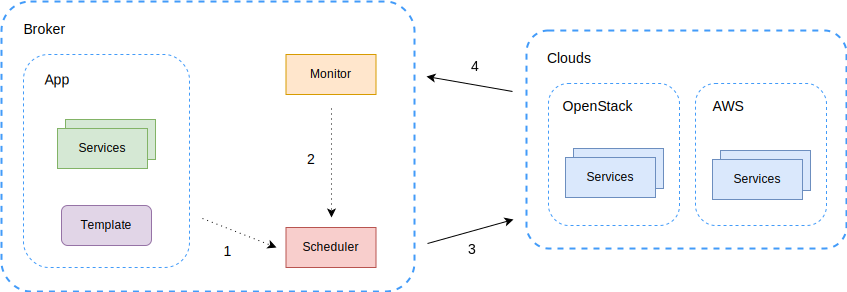
\includegraphics[width=\linewidth]{images/broker-cycle}
	\caption{Vereinfachte Arbeitsweise des Multi-Cloud-Brokers als Regelkreis: (1) Sammeln der SLAs, Anwendungsvorlagen und Nutzeränderungen (2) Sammeln der Metainformationen aller Cloud-Provider, (3) Optimierungsplanung und Ausführung auf den Cloud-Infrastrukturen, (4) Sammeln der Laufzeitinformationen der Anwendungen.}
	\label{fig:cycle}
\end{figure}

%Ausführlicher Regelkreis mit einzelnen Parametern und Teilschritten.
\begin{minipage}[b]{0.45\linewidth}
\begin{flushleft}
\begin{enumerate}
\item Monitoring Cloud-Ressourcen
\begin{enumerate}
	\item Kapazität% (CPU, RAM, HDD, Netzwerk)
	\item Features% (Verschlüsselung, CUDA, \ldots)
	\item Geo-Lokation
	\item Preis
\end{enumerate}
\item Laufzeitinformationen% der PaaS/Anwendungen
\begin{enumerate}
	\item Auslastung
	\item Fehler
	\item Ausfälle
\end{enumerate}
\item Sammeln der SLAs
\begin{enumerate}
	\item Policy-Definitionen
	\item Policy-Konfiguration
	\item Placement-Algorithmen
\end{enumerate}
\end{enumerate}
\end{flushleft}
\end{minipage}
%
\hspace{0.5cm}
%
\begin{minipage}[b]{0.45\linewidth}	
\begin{enumerate}
\setcounter{enumi}{3}
\item (Neue Anwendung)
\item (Änderung von SLAs)
\item Optimierung
\begin{enumerate}
	\item Feste Vorgaben% (Geo, Backup)
	\item Weiche Kriterien% (Preis, Latenz, Verfügbarkeit)
\end{enumerate}
\item Ausführung
\begin{enumerate}
	\item Netzwerkkonfiguration
	\item Allokation/De-Allokation von Ressourcen
	\item Deployment
	\item Migration
	\item Logging% und \newline Benachrichtigung
	\item Backup
\end{enumerate}
\end{enumerate}
\end{minipage}

\vspace{0.5cm}

\noindent
Aus der abstrakten Definition der Komponenten und des Brokeringmechanismus lässt sich noch nicht ganz ein Prototyp bauen. Zusätzlich benötigen wir eine formale Definition der Cloudzugangsdaten, Anwendungen und SLAs. Nach deren Einführung beschreiben wir Multi-Cloud-Bibliotheken und anschließend die Implementierung.
